\chapter{System Design}
Provide a detailed explanation of the overall system architecture \cite{lin1991divergence}, i.e. the HOW of the project.
Use UML, system architecture diagrams, screenshots, code snippets and algorithms to illustrate your design.

\section{Working with Images}
You can embed an image in a \LaTeX document using the technique shown below. System diagrams and images with a small numbers of colours (100s, not 1000s) should be stored in PNG format. Although \LaTeX doesn't care where you place your images, it is good practice to place them in a single sensible directory and apply some sort of hierarchy to them, e.g. the path images/chapter1 might contain all of the images for Chapter 1 of your dissertation.

\begin{figure}[h!]
    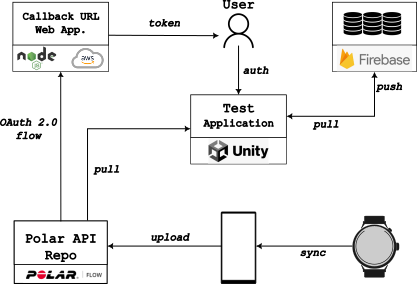
\includegraphics[width=0.9\textwidth]{images/architecture.png}
    \caption{System Architecture.}
    \label{image:sysArchitecture}
\end{figure}

Image \ref{image:sysArchitecture} can be referenced with the label given to the image, \\ i.e. \textbf{\textbackslash{}ref\{image:sysArchitecture\}}. Note that \LaTeX will place the image wherever it deems fit. Don't bother trying to change where a table or figure is placed until your document is ready for final layout.